\documentclass[12pt]{article}
\usepackage[a4paper]{geometry}
\usepackage[spanish,es-tabla]{babel}
\usepackage[utf8]{inputenc}
\usepackage[T1]{fontenc}
% \usepackage{fontspec}
\usepackage{graphicx}
\usepackage{times}
\usepackage{tipa}
\usepackage{amsmath}
\usepackage{setspace}
\usepackage{enumitem}
\usepackage{fancyhdr}
\usepackage{lipsum}
\usepackage{parskip}
\usepackage[backend=biber, style=apa]{biblatex}
\addbibresource{bibliografia.bib}
\usepackage{caption}
\usepackage{floatrow}
\usepackage{titlesec}
\usepackage{titletoc}
\usepackage{appendix}
\usepackage{tabularray}
\usepackage{tocloft} 
\usepackage{physics}
\usepackage{changepage}
\usepackage[hidelinks]{hyperref} % eliminar rectangulos rojos en los links

\usepackage{titlesec}
\titleformat{\section}
  {\normalfont\fontsize{16}{16}\bfseries}{\thesection .}{0.5ex}{}
\titleformat{\subsection}
  {\normalfont\fontsize{14}{14}\bfseries}{\thesubsection .}{0.5ex}{}
\titleformat{\subsubsection}
  {\normalfont\fontsize{14}{14}\bfseries}{\thesubsubsection.}{0.5ex}{}
\titleformat{\paragraph}
{\normalfont\normalsize\bfseries}{\theparagraph}{1em}{}
\titlespacing*{\paragraph}
{0pt}{3.25ex plus 1ex minus .2ex}{1.5ex plus .2ex}

%-----------------CONFIGURACION-------------------------------

% Configuracion de la Pagina 
\geometry{
    a4paper,
    total={21cm,29.7cm},
    left=3cm,
    top=2.5cm,
    right=2.5cm,
    bottom=2.5cm }

\setstretch{1.5} %Interlineado a 1.5
\setlength{\parindent}{1cm} %Sangría de cada nuevo párrafo a 1cm

% Configuración del pie de página
\fancyfoot[C]{\rule{\textwidth}{0.4pt}\\ \hspace*{\fill}\fontsize{12pt}{14pt}\selectfont Desarrollo de sistema automático de audiolibros con voces de la cultura argentina. \hspace*{\fill}\thepage} 

%\setlength{\footskip}{1.02 cm}
\setlength{\footskip}{0.5 cm}
\pagestyle{fancy} % Establecer el estilo de página como 'fancy'

\fancyhead{} % Limpiar encabezado
\renewcommand{\headrulewidth}{0pt} % Eliminar la línea de encabezado

\DefineBibliographyStrings{spanish}{ % Redefinir la cadena de texto para Bibliografía
  references = {BIBLIOGRAFÍA}, % <-- Aquí cerramos correctamente la definición}

% Configuración global de las descripciones de las figuras
\captionsetup[figure]{labelsep=period}
% Configuración global de las descripciones de las tablas
\floatsetup[table]{capposition=top}
\captionsetup[table]{labelsep=period}

% Personalización del formato del índice de figuras
\renewcommand{\cftfigpresnum}{Figura }
\renewcommand{\cftfigaftersnum}{.}
\setlength{\cftfignumwidth}{4em}

% Personalización del formato del índice de tablas
\renewcommand{\cfttabpresnum}{Tabla }
\renewcommand{\cfttabaftersnum}{.}
\setlength{\cfttabnumwidth}{4em}

% Personalizar el formato del índice general
\renewcommand{\cftsecleader}{\cftdotfill{\cftdotsep}} % Agrega puntos entre el título de la sección y el número de página
\renewcommand{\cftsecfont}{\bfseries} % Establece la fuente del título de la sección en el índice como negrita
\renewcommand{\cftsecpagefont}{\bfseries} % Establece la fuente de la página de la sección en el índice como negrita


% Definir el espaciado entre sections y subsections
\titlespacing*{\subsection}{1cm}{*1.5}{*1}

% Definir el espaciado entre subsections y subsubsections
\titlespacing*{\subsubsection}{1.5cm}{*1.5}{*1}

\usepackage{fontspec}
\setromanfont[
BoldFont=Calibri Bold.TTF,
ItalicFont=Calibri Italic.ttf,
BoldItalicFont=Calibri Bold Italic.ttf,
]{Calibri Regular.ttf}

\begin{document}

%-------------------------- PORTADA -----------------
\begin{titlepage}
\centering

\includegraphics[width=13.58cm, height=3.1cm]{Logo Untref.png} 

\vspace{0.1cm}

\hspace*{-1.31cm}% Espacio horizontal de 1.31cm desde el borde izquierdo de la hoja
\begin{minipage}[t]{16cm}
\centering
\framebox[17.13cm][c]{\parbox{18.13cm}{\centering{\fontsize{16pt}{1.5pt}\selectfont INGENIERÍA DE SONIDO}}}
\vspace{0.5cm} % Espacio vertical entre el recuadro y el texto siguiente

\end{minipage}


\vspace{36pt}

{\bfseries\fontsize{22pt}{18pt} \selectfont Desarrollo de sistema automático de audiolibros con voces de la cultura argentina. \par}

\vspace{42pt}

% {\itshape\fontsize{18pt}{24pt}\selectfont \textbf{Subtítulo de la tesis (si lo tuviera)} \par}

\vspace{64pt}

{\centering\itshape\fontsize{14pt}{1pt}\selectfont Tesis final presentada para obtener el título de Ingeniero\par}
{\centering\itshape\fontsize{14pt}{1pt}\selectfont de Sonido de la Universidad Nacional de Tres de Febrero \par}
{\centering\itshape\fontsize{14pt}{1pt}\selectfont (UNTREF) \par}

\vspace{70pt}

{\bfseries\fontsize{14pt}{0pt}\selectfont TESISTA: Nahuel Passano (DNI: 40.910.030) \par}
{\bfseries\fontsize{14pt}{0pt}\selectfont TUTOR: Ing. Leonardo Pepino \par}
{\bfseries\fontsize{14pt}{0pt}\selectfont COTUTOR: Ing. Ignacio Mieza \par}

\vfill

\begin{table}[h]
\hrulefill \\ 
\begin{tabular}{c}
Fecha de defensa: mes y año $\lvert$ Locación: Buenos Aires, Argentina \\
\end{tabular}
\end{table}
\hrule
\end{titlepage}

\newpage
\thispagestyle{empty} % Página en blanco sin número de página, encabezado ni pie de página
\mbox{} % Contenido de la página en blanco
\newpage

%---------------------------------------------------------------
% CUERPO DEL DOCUMENTO
% Centrar título de sección

\pagenumbering{roman} % Comienza la numeración de página en números romanos
\setcounter{page}{2} % Establece el número de página según sea necesario
\setcounter{secnumdepth}{4}
%-----------------Agradecimientos-----------------
\newpage 
\thispagestyle{plain} 
% \section*{AGRADECIMIENTOS} % Título centrado
\begin{centering}
\Large{\textbf{AGRADECIMIENTOS}}

\end{centering}

Se propone incluir este apartado, donde se debe agradecer primeramente a las autoridades de la Universidad, al coordinador de la carrera, al tutor y a los docentes implicados en el desarrollo de la investigación. Seguidamente agradecer a familiares o a aquellas personas que se quiera. También puede incluirse en la siguiente hoja una dedicatoria personal. A modo de ejemplo el contenido podría ser:

“En primer lugar dar gracias a la Universidad Nacional de Tres de Febrero (UNTREF), a su Rector Emérito Lic. Anibal Jozami y Rector Lic. Martín Kaufmann, a todo su personal docente y no docente. Por promover un espacio ideal para el desarrollo de ideas y nuevos pensamientos y brindar a todos y cada uno de los alumnos, de esta casa de altos estudios, todos los recursos que esta institución dispone.   
Esta investigación no hubiera sido posible sin una formación académica acorde, por este motivo debo extender mi agradecimiento a los docentes de la carrera de Ingeniería de Sonido de la UNTREF, a su coordinador Ing. Alejandro Bibondo, que siendo la primera carrera de estas características del país, es muy importante contar con un cuerpo docente afín a las exigencias que este desafío propone, prestando su dedicación y vocación de enseñar. 
Un especial agradecimiento por la participación de esta tesis a la tutora Ing. Nombre Apellido, que supo transmitirme sus conocimientos y ayudarme a organizarme y fijarme un rumbo concreto y delineado, disponiendo desmedidamente de su tiempo. 
Por otra parte, quisiera hacer una mención especial al Ing. Hernan San Martin, que permitió el uso de las instalaciones de su laboratorio para poder trabajar y la disposición de todos sus recursos para que dicha investigación se realizara en tiempo y forma. 
Por último y no menos importante, quiero dar un afectuoso y cálido agradecimiento a mi familia…”


\newpage


\clearpage

\newpage
\thispagestyle{plain} % Página en blanco sin número de página, encabezado ni pie de página
\mbox{} % Contenido de la página en blanco
\newpage

%-----------------Estado del Arte-----------------
\newpage
\thispagestyle{plain} 
% \section*{DEDICATORIA} 
\textcolor{white}{
hola \\
hola \\
hola \\
hola \\
}
\begin{flushright}
\LARGE{\textbf{DEDICATORIA}}
\end{flushright}


\begin{flushright}
\textit{Elige a quién o a qué quieres dedicárselo \\
Elegir el motivo de la dedicatoria (orientativo)
}
\end{flushright}


%------------------Indices------------------------
\newpage
\renewcommand{\contentsname}{ÍNDICE DE CONTENIDOS}
\tableofcontents   % Índice General
\listoffigures  % Índice de Figuras
\listoftables   % Índice de Tablas 


%------------------Resumen------------------------

\newpage
\thispagestyle{plain} 
% \section*{\centering RESUMEN} 
\addcontentsline{toc}{section}{RESUMEN} % Agregar RESUMEN al índice
\begin{centering}
\Large{\textbf{RESUMEN}}

\end{centering}

% \raggedright
Su contenido no debe superar una página. Se indicarán los objetivos del trabajo, los métodos y resultados principales. A dos espacios debajo del resumen, en la misma página, se colocarán hasta 5 palabras clave que identifican los contenidos del trabajo.



\textbf{Palabras Clave:} 

% \end{titlepage}

%------------------Abstrac------------------------

\newpage
\thispagestyle{plain} 
% \section*{\centering ABSTRACT} 
\addcontentsline{toc}{section}{ABSTRACT} % Agregar ABSTRACT al índice
\begin{centering}
\Large{\textbf{ABSTRACT}}

\end{centering}

Ídem que para castellano. \\

\textbf{Keywords:} 




%-----------------Introducción-----------------
\clearpage % Asegúrate de que la sección de introducción comience en una nueva página
\pagenumbering{arabic} % Restaurar numeración arábiga
\section{INTRODUCCIÓN} 
\subsection{Fundamentación}

La evolución tecnológica y la adopción de nuevas tecnologías han marcado un punto de inflexión en la producción de contenido digital. Específicamente, la integración de la inteligencia artificial en la creación de imágenes, videos y audio ha desencadenado una revolución significativa en términos de calidad, técnicas y velocidad de generación de nuevo contenido. Ante este panorama, la necesidad de adaptar y mejorar continuamente los métodos de producción se ha vuelto imperativa. La creciente demanda de accesibilidad y personalización en los medios digitales impulsa la búsqueda de soluciones innovadoras que no solo optimicen los procesos existentes sino que también abran nuevas vías para la creación de material. 
En este contexto, los audiolibros emergen como un medio particularmente relevante, dada su creciente popularidad y su capacidad para ofrecer una experiencia complementaria e innovadora a la lectura tradicional. Sin embargo, el desarrollo de audiolibros presenta desafíos singulares. En primer lugar, se necesita contratar a un narrador capaz de cautivar con sus historias. Además, para ofrecer una experiencia más inmersiva, es necesario grabar en un entorno acústicamente controlado, utilizando equipos profesionales como micrófonos de alta fidelidad y una placa de audio de calidad. Por último, se requiere un trabajo de post-producción realizado por un especialista. Estos requisitos implican que la producción conlleva una inversión significativa, tanto en términos financieros (para la contratación del narrador y los profesionales encargados de la grabación) como en cuanto al tiempo necesario. Ante este panorama, se propone investigar el diseño e implementación de un sistema automatizado de generación de audiolibros, el cual se centra principalmente en producir narraciones naturales y de alta calidad. Este sistema busca abordar dichos desafíos mediante el aprovechamiento de las últimas innovaciones en inteligencia artificial aplicada al procesamiento digital de señales, representando un paso adelante significativo en el campo. La integración de estas tecnologías no solo permitirá una producción más eficiente, personalizable y rápida, sino que también mejorará la calidad del producto final, proporcionando una herramienta capaz de narrar textos con la fluidez de un locutor profesional. La generación de voz sintética, en particular, se basa en modelos de aprendizaje profundo que pueden capturar las inflexiones y emociones humanas, ofreciendo una experiencia auditiva agradable y reconfortante. Por otro lado, el procesamiento digital de señales juega un papel crucial en la mejora de la claridad y la calidad del habla, además de ser una herramienta fundamental en el preprocesamiento y postprocesamiento de los audios a utilizar. Otro desafío significativo en el presente desarrollo es la adaptación tecnológica al idioma español, específicamente al dialecto rioplatense. Aunque existen numerosos sistemas capaces de sintetizar discursos en un español nativo, la capacidad para abordar las diversas variantes y dialectos del español es limitada. Por lo tanto, esta investigación se centra en la creación de una herramienta que logre representar y narrar historias incorporando los elementos característicos del dialecto rioplatense, tales como el yeísmo, su particular ritmo y sus marcadores de identidad. Por último, se propone incorporar como narradores a figuras destacadas de la cultura argentina, con el objetivo de generar identificación e impacto en los potenciales usuarios de la plataforma.


\subsection{Objetivos}

\subsubsection{Objetivo general}

El objetivo principal de esta investigación es desarrollar una herramienta de acceso libre que permita la generación de audiolibros personalizables con voces reconocidas de la cultura  argentina.

\subsubsection{Objetivos específicos}

\begin{itemize}
    \item Recopilar discursos de figuras icónicas de Argentina, seleccionando las voces más distintivas y reconocidas de su cultura.
    \item Crear una plataforma de preprocesamiento de audio que facilite la obtención de oraciones y sus transcripciones automáticas.
    \item Conformar una base de datos idónea para el entrenamiento y ajuste del sistema con la plataforma diseñada.
    \item Implementar un sistema de validación para las transcripciones automatizadas, asegurando un control riguroso de la calidad de los audios y sus correspondientes transcripciones.
    \item Realizar un ajuste fino del modelo para emular las voces seleccionadas.
    \item Llevar a cabo encuestas subjetivas para evaluar la calidad, naturalidad y similitud de las narraciones generadas.
    \item Utilizar métricas objetivas que complementen las evaluaciones subjetivas recogidas.
    \item Comparar los resultados obtenidos con investigaciones previas para evaluar objetiva y subjetivamente el desempeño del sistema.
    \item Proveer una plataforma de acceso libre que permita el uso del servicio desarrollado.

\end{itemize}

\subsection{Estructura de la investigación}

En el capítulo 2 se presenta una revisión meticulosa del estado del arte y la construcción del marco teórico detallado. Este marco abarca estudios previos y desarrollos tecnológicos en áreas clave. Se destacan tanto las soluciones existentes como las limitaciones actuales, estableciendo un contexto para la innovación propuesta y asegurando que el diseño e implementación del sistema consideren las mejores prácticas y los hallazgos más recientes. 

En el capítulo 3 se describe el paso a paso en el desarrollo de la herramienta, detallando etapas claves como la recolección y conformación del conjunto de datos a utilizar, el entrenamiento y ajuste del sintetizador elegido y el diseño de la plataforma que será utilizada por los usuarios finales.

En el capítulo 4 se comenta como se evalúa el sistema desarrollado, describiendo tanto su evaluación objetiva como subjetiva. En el mismo se detallan las métricas a utilizar, las cuales intentan cuantificar distintas características de los discursos sintéticos generados, como lo son la naturalidad, la calidad y la similitud con la voz objetivo. A su vez, se describe el proceso para evaluar el sistema desde una perspectiva subjetiva con una prueba del tipo Mean Opinion Score (MOS).

En el capítulo 5 se lleva a cabo una validación en términos estadísticos y metodológicos de la muestra recolectada en la prueba subjetiva, describiendo los métodos para su análisis y ...

En el capítulo 6 se realiza el análisis de los resultados, donde se nuclea los análisis realizados en los capítulos 4 y 5 en pos de tener una representación real del rendimiento del sistema (sanata).

En el capítulo 7 se realizan las conclusiones finales del sistema desarrollado, marcando los hitos de todo el desarrollo y los aspectos que pueden ser mejorados.

En el capitulo 8 se esbozan ideas y propuestas para líneas futuras de investigación, donde se intenta un panorama general de las mejoras del sistema, así como la dirección de investigación en el estado del arte actual. (sanata)



\clearpage



%-----------------Marco Teorico-----------------
\newpage
\section{MARCO TEÓRICO Y ESTADO DEL ARTE} 
    En esta sección, se procede a detallar los fundamentos esenciales que configuran la base conceptual y metodológica de la presente investigación. Inicialmente, se ofrece una breve introducción sobre las diversas formas de representar un audio. Posteriormente, se describe de forma básica que son los algoritmos de aprendizaje profundo basados en redes neuronales artificiales, definiendo los conceptos principales que se requieren para interpretar y entender como se entrenan estos modelos y fundamentar las fases del desarrollo propuesto. A su vez, se realiza una revisión de  la historia de la síntesis de voz, pasando desde los primeros sistemas de síntesis articulatoria, hasta llegar a los sistemas basados en redes neuronales. Por último, se realiza un minucioso análisis de dos sistemas específicos que son objeto de comparación en esta investigación, complementado con una comparación con otros modelos presentes en el estado actual del arte.

\subsection{Representaciones de audio}

En el desarrollo de algoritmos aplicados al procesamiento digital de señales, es muy importante conocer las distintas formas que se utilizan para representar un audio. Debido a la naturaleza del proceso de muestreo y digitalización, la representación más elemental e intuitiva es en el dominio temporal, ofreciendo información sobre la amplitud de la señal en función del tiempo. Esta representación es útil para visualizar la forma de onda y la duración de los distintos eventos sonoros. 

\begin{figure}[h]
    \centering
    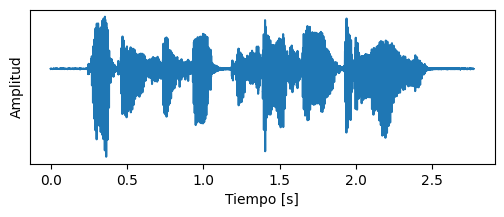
\includegraphics[width=0.75\textwidth]{figures/2.1.waveform.png}
    \caption{Representación de un discurso en el dominio temporal}
    \label{fig:2.1. waveform}
\end{figure}

Por otro lado, la representación en el dominio frecuencial permite visualizar y analizar como se distribuye la energía en el espectro de frecuencias. 

\begin{figure}[h]
    \centering
    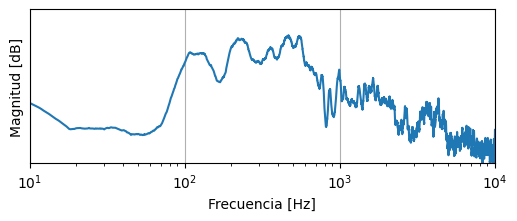
\includegraphics[width=0.75\textwidth]{figures/2.1.spectrum.png}
    \caption{Representación de un discurso en el dominio frecuencial}
    \label{fig:2.1. spectrum}
\end{figure}

Al utilizar la representación temporal del audio, si bien se pueden observar fenómenos energéticos y localizar los mismos en el tiempo, no se puede discernir con solo visualizar la forma de onda si dos señales tienen la misma información o no. Asimismo, al analizar únicamente la representación frecuencial, se pierde la información temporal, la cual es crucial para comprender la dinámica y evolución de la señal a lo largo del tiempo. Para aprovechar la información proporcionada por ambas representaciones, se utilizan las representaciones del tipo tiempo-frecuencia, las cuales permiten analizar cómo evolucionan y cambian los eventos sonoros tanto temporal como frecuencialmente. La representación mas conocida de este tipo es el espectograma, el cual se obtiene a partir de la transformada de Fourier de tiempo corto (STFT, por sus siglas en inglés Short-Time Fourer Transform).


\subsubsection{Transformada de Fourier de tiempo corto (STFT)}
La transformada de Fourier de tiempo corto (STFT) es utilizada para determinar el comportamiento frecuencial y temporal de una señal (\cite{sejdic2009}). En la práctica, el procedimiento para calcular la STFT consiste en tomar pequeños segmentos de la señal a analizar y calcular la transformada de Fourier discreta (DFT, por sus siglas en ingles Discrete Fourier Transform) para cada segmento. Luego, los resultados de la DFT aplicada a cada segmento se agrupan en una matriz compleja, donde las filas representan los bines de frecuencia, y las columnas los segmentos temporales en los que se calculó la DFT. Dado que la transformada de Fourier discreta aplicada a una señal da como resultado una señal compleja, la matriz de la STFT será, a su vez, una matriz compleja. El procedimiento de cálculo tiene algunos detalles y parámetros importantes que modifican el resultado de la transformada, los cuales son:


\begin{itemize}
    \item \textbf{Tamaño de segmento ($M$)}: Todos los segmentos tienen la misma cantidad de muestras, y en base a este parámetro surge una importante relación de compromiso. A medida que se incrementa la cantidad de muestras por segmento, se obtiene una mayor resolución en frecuencia, pero menor resolución temporal, y en contrapartida, al reducir la cantidad de muestras por segmento, se obtiene una mayor resolución temporal a costa de una menor resolución en frecuencia. Generalmente se utilizan valores que sean potencia de 2 (256, 512, 1028) para agilizar el cálculo de la FFT.
    \item \textbf{Tipo de ventana ($w[n]$)}: El procesamiento de los segmentos se suele realizar con un ventaneo previo para evitar los artefactos producidos en los bordes de cada bloque por la discontinuidad de fase. Generalmente se suele utilizar la ventana de Hann.
    \item \textbf{Tamaño de salto ($h$)}: Los segmentos suelen tener un cierto porcentaje de solapamiento en pos de no perder información en sus bordes por culpa del ventaneo. En la práctica, el solapamiento se suele cuantificar con el tamaño de salto entre segmentos (en ingles se conoce como \textit{hop size}). Generalmente se utilizan segmentos con un 50\% de solapamiento, es decir, un tamaño de salto que es la mitad del tamaño de bloque.
\end{itemize}

En la figura \eqref{fig:2.1.stft} se puede ver como interactúan los parámetros mencionados en el procedimiento de cálculo.

\begin{figure}[h]
    \centering
    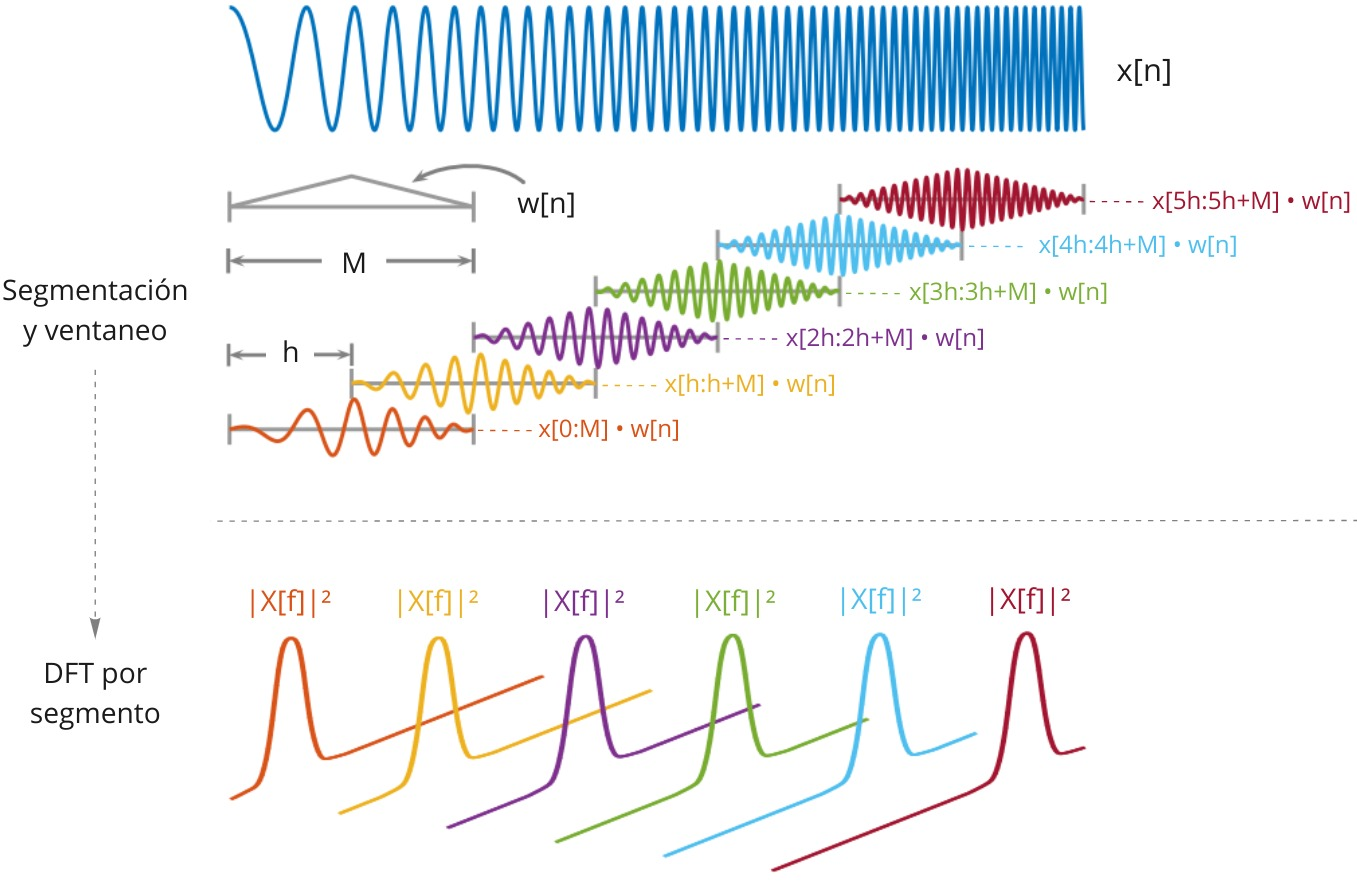
\includegraphics[width=0.95\textwidth]{figures/2.1.stft.jpg}
    \caption{Procedimiento de cálculo de la STFT}
    \label{fig:2.1.stft}
\end{figure}


Matemáticamente, la STFT para una señal discreta $x[n]$ de $M$ muestras se calcula según la ecuación \eqref{eq: stft}:

\vspace{-10mm}

\begin{equation}
    STFT\{x[n]\} = X[k, seg] = \sum \limits_{seg=0}^{N_{seg}} \underbrace{\sum \limits_{k=0}^{M-1} w[n] ~ x[seg\cdot h:seg\cdot h + M] ~ e^{-j2\pi k n / M}}_{\textit{DFT por segmento}}
    \label{eq: stft}
\end{equation}

Por último para obtener el espectrograma de una señal, se debe elevar al cuadrado la magnitud de la STFT ($|X[k, seg]|^2$). Este tipo de representación es de gran utilidad para localizar eventos sonoros tanto temporal como frecuencialmente, pero la mayor información de la voz humana queda concentrada en un rango pequeño del eje frecuencial como se puede ver en la figura \eqref{fig:2.1.spectogram}.

\begin{figure}[h]
    \centering
    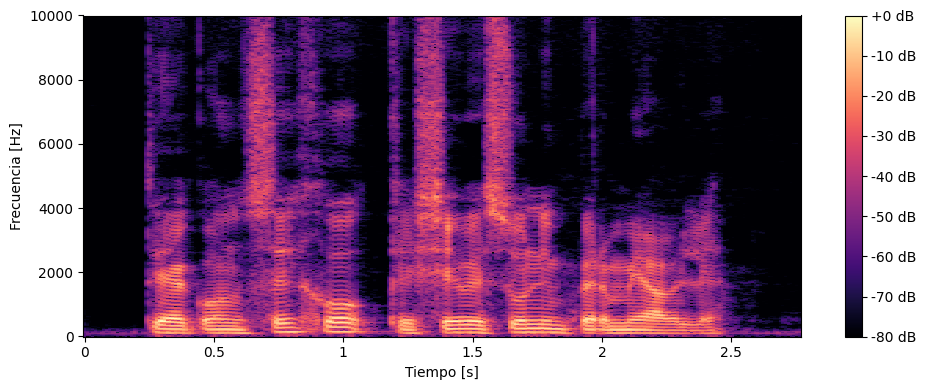
\includegraphics[width=0.85\textwidth]{figures/2.1.spectogram.png}
    \caption{Espectograma del discurso presentado en las figuras \eqref{fig:2.1. waveform} y \eqref{fig:2.1. spectrum}} 
    \label{fig:2.1.spectogram}
\end{figure}

\subsubsection{Espectograma de Mel}

El espectrograma de Mel, similar al espectrograma convencional, es una representación de la energía de una señal de audio en relación con el tiempo y la frecuencia. Sin embargo, se distingue por el mapeo de frecuencias según la escala de Mel, una escala perceptual que refleja cómo los seres humanos perciben las variaciones de tono entre diferentes sonidos. El mapeo para convertir  las frecuencias de la escala convencional $f$ en las frecuencias de la escala Mel $m$ se describe en la ecuación \eqref{eq:2.1.mel_scale}.

\begin{equation}
    m = 2595\log_{10} \Big ( 1 + \frac{f}{700} \Big )
    \label{eq:2.1.mel_scale}
\end{equation}

En la figura \eqref{fig:2.1.mel-spectogram} se puede visualizar el espectograma de Mel aplicado a una señal de habla. En comparativa con el espectograma convencional de la figura \eqref{fig:2.1.spectogram}, se puede notar que se resalta mas el contenido armónico del habla. Este tipo de representación es mas adecuada para  analizar habla ya que se puede observar con mas detalle el rango frecuencial en donde se ubica la voz humana.


\begin{figure}[h]
    \centering
    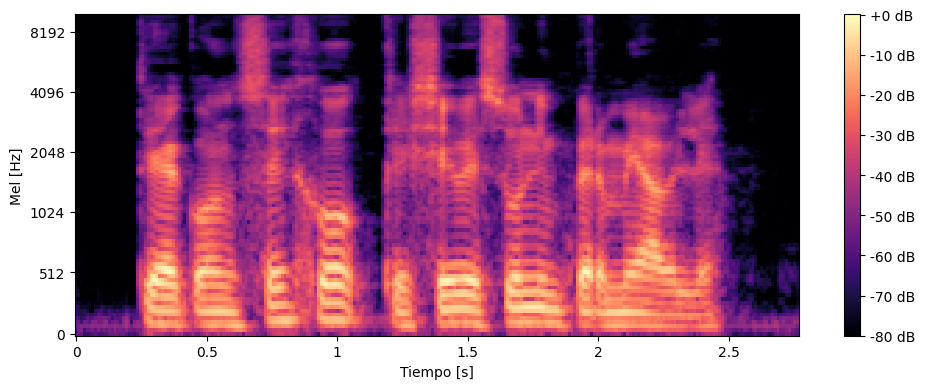
\includegraphics[width=0.85\textwidth]{figures/2.1.mel-spectogram.png}
    \caption{Espectograma de Mel del discurso presentado en las figuras \eqref{fig:2.1. waveform} y \eqref{fig:2.1. spectrum}} 
    \label{fig:2.1.mel-spectogram}
\end{figure}

\subsection{Algoritmos de aprendizaje profundo y redes neuronales artificiales}
Dentro de los algoritmos de aprendizaje profundo, una red neuronal artificial es un modelo matemático inspirado en la estructura y funcionamiento de las neuronas biológicas (\cite{hardesty2017}). En la actualidad, su aplicación se extiende por diversas ramas de la ciencia, y su adopción para la resolución de problemas ha experimentado un crecimiento exponencial en tiempos recientes.

\subsubsection{Neurona artificial}
Una red neuronal artificial se compone de nodos llamados neuronas artificiales, las cuales están interconectadas entre si emulando el proceso de sinapsis (\cite{basheer2000}). En la figura \eqref{fig:2.2.neuron} se puede ver un esquema de los elementos que componen a cada neurona dentro de una red. Cada neurona recibe una determinada señal, la cual procesa y envía a la neurona siguiente. La señal que recibe es una \textbf{serie de números reales} $x_n$, y la salida de cada neurona se calcula mediante una función no lineal aplicada a la suma ponderada de sus entradas, llamada \textbf{función de activación}. La fuerza de la señal en cada conexión es determinada por un \textbf{peso}, que se ajusta durante el proceso de aprendizaje. A su vez, se introduce un término de \textbf{bias} a la suma ponderada, el cual también se actualiza en el proceso de entrenamiento.

\begin{figure}[h]
    \centering
    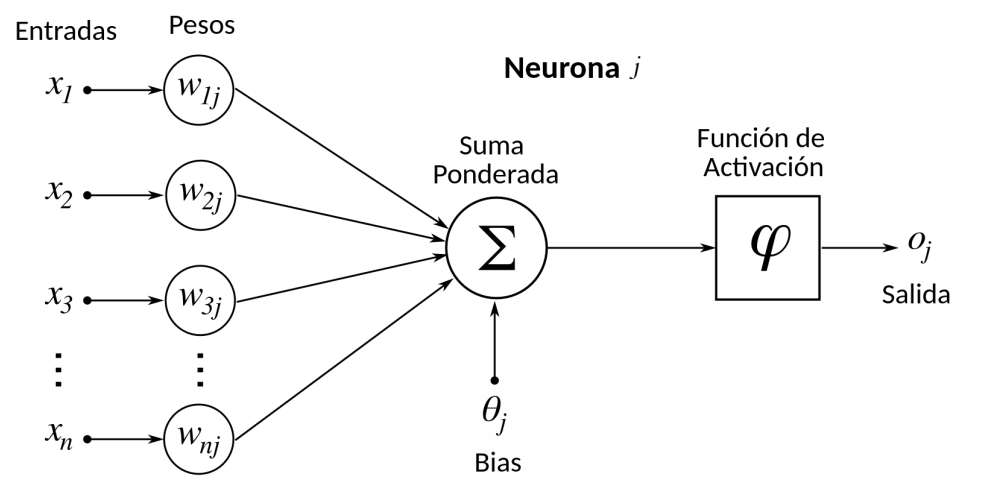
\includegraphics[width=0.85\textwidth]{figures/2.2.neuron.png}
    \caption{Esquema de una neurona artificial} 
    \label{fig:2.2.neuron}
\end{figure}

Este proceso se puede describir matemáticamente con la ecuación \eqref{eq: neuron}.

\begin{equation}
    o_j = \varphi \Big ( \sum \limits_{i=1}^{n}x_i w_{ji} + \theta_j \Big )
    \label{eq: neuron}
\end{equation}

\subsubsection{Redes neuronales artificiales}
Por lo general, las neuronas artificiales se agrupan en \textbf{capas}. Las señales se propagan desde la primera capa (la capa de entrada) hasta la última capa (la capa de salida), pasando por múltiples capas intermedias (capas ocultas). Una red se suele llamar \textbf{red neuronal profunda} si tiene al menos 2 capas ocultas. Esto se debe a que contienen múltiples capas de procesamiento no lineal que aprenden diferentes niveles de representación formando una jerarquía de características, desde un nivel de abstracción más bajo a uno más alto (\cite{chollet2021}). A la hora de construir y diseñar una red neuronal es necesario definir una serie de parámetros que caracterizan como se propaga la señal desde la entrada hasta la salida, como por ejemplo la cantidad de capas, cantidad de neuronas por capa, las funciones de activación, entre otros. Estos parámetros son conocidos como \textbf{hiperparámetros}, ya que se definen a la hora de construir la red pero no se modifican en el proceso de entrenamiento. En la figura \eqref{fig:2.2.net} se puede ver el esquema de una red neuronal profunda básica, la cual está compuesta por 4 capas, una de entrada con 3 neuronas, dos capas ocultas con 5 y 4 neuronas respectivamente, y una de salida con 2 neuronas. Este tipo de red es conocida como perceptron multicapa (\cite{hornik1991}), y a cada nodo se lo denomina perceptron. 


\begin{figure}[h]
    \centering
    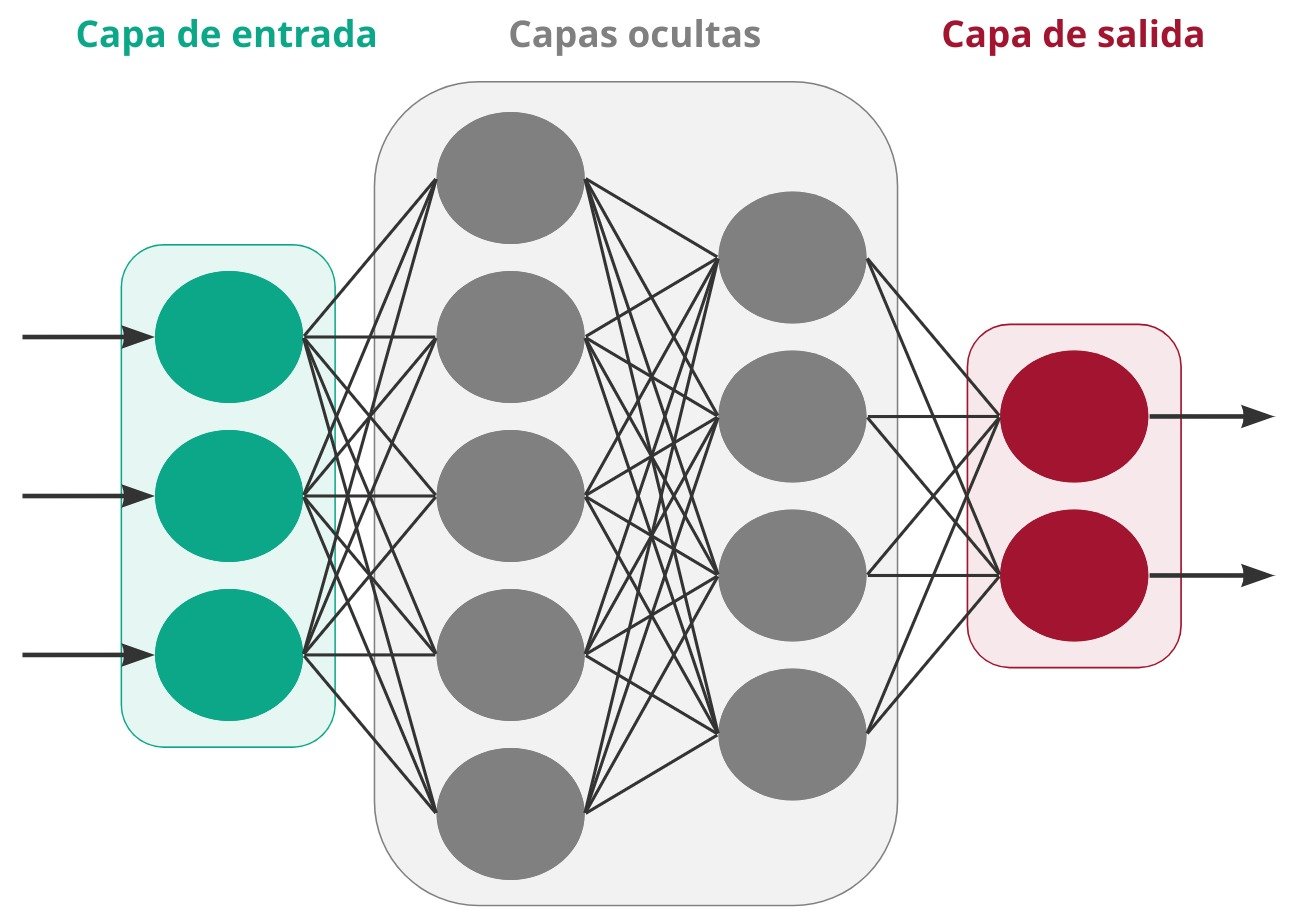
\includegraphics[width=0.7\textwidth]{figures/2.2.net.png}
    \caption{Ejemplo de una red neuronal profunda} 
    \label{fig:2.2.net}
\end{figure}

\subsubsection{Entrenamiento y optimización de modelos}

Los modelos basados en redes neuronales artificiales se dice que ''aprenden'' de los datos producto de un entrenamiento. Este entrenamiento no es mas que un proceso de optimización en el cual se busca que las predicciones del modelo sean lo mas parecidas y cercanas a los valores esperados. Existen diversas formas en las que un modelo puede aprender, siendo la más común denominada aprendizaje supervisado. En este enfoque, los datos de entrenamiento consisten en ejemplos etiquetados que indican cómo debería comportarse el modelo. Esto significa que se le proporciona al modelo tanto los datos de entrada $x$ como las respuestas deseadas $y$ correspondientes. El objetivo es que el modelo aprenda a mapear las entradas a las salidas correctas. En el contexto del entrenamiento de una red neuronal, se define al aprendizaje como la búsqueda de una determinada configuración de los parámetros entrenables $W$ de la red que produzcan que la entrada $x$ genere la salida $y$. En general, al inicio del entrenamiento las entradas van a generar salidas $\hat{y}$ aleatorias que difieren del valor objetivo $y$. Por lo tanto, es necesario tener una medida de esta diferencia. De eso se encarga la función de costo $\mathcal{L}$ (también denominada función de pérdida).

{\large \textbf{Función de costo $\mathcal{L}$}}


La función de costo recibe las salidas de la red $\hat{y}$ y las salidas esperadas $y$, y luego calcula una medida de error a partir de una función matemática. Una de las funciones de costo más conocidas y utilizadas es el error cuadrático medio (MSE, por sus siglas en inglés, Mean Squared Error), que se caracteriza mediante la ecuación \eqref{eq:mse}.

\begin{equation}
    \mathcal{L}(y,\hat{y}) = \frac{1}{N}\sum \limits_{i=1}^{N} (y - \hat{y})^2
    \label{eq:mse}
\end{equation}

La selección de esta función se basa en la característica que se desea analizar y comparar entre las predicciones y los valores esperados. Por lo tanto, para cada estimación de la red, la función de costo otorga un puntaje que explica cuan lejos está el valor estimado del valor objetivo. 

{\large \textbf{Optimización y propagación del error}}

El paso siguiente en el proceso de entrenamiento es utilizar la salida de la función de costo como una señal de realimentación para poder ajustar los parámetros entrenables $W$ de la red neuronal de manera tal de minimizar la función de costo. Esta tarea es realizada por la función de optimización. La misma aplica el algoritmo de propagación del error hacia atrás para computar el gradiente de la función de costo respecto a los parámetros entrenables $W$ de la red. Desde una perspectiva matemática, el gradiente se define como un vector que apunta hacia el punto de máximo crecimiento de una función, mientras que su sentido contrario indica el punto de mínimo crecimiento. Por lo tanto, para minimizar la función de pérdida, es necesario ajustar los parámetros en la dirección opuesta al vector gradiente. A su vez, la fuerza con la que se modifican los parámetros en la dirección opuesta del gradiente se llama tasa de aprendizaje $\eta$. Una vez calculado el gradiente y definida la tasa de aprendizaje $\eta$, se puede determinar cómo modificar los parámetros entrenables $W$ con el fin de reducir el error de salida. Esta operación se puede ver expresada en la ecuación \eqref{eq:learning_rate}.

\begin{equation}
    W := W - \eta \cdot \frac{\partial ~\mathcal{L}}{\partial W}
    \label{eq:learning_rate}
\end{equation}

{\large \textbf{Procesamiento del conjunto de datos}}

En la etapa de entrenamiento, el modelo procesa el conjunto de datos por lotes, es decir, en cada iteración de entrenamiento se toma una muestra sin reposición de un determinado tamaño, se procesa, se calcula la pérdida con la función de costo y
ajusta los parámetros de cada capa. Cuando la red procesó todos los lotes que componen el conjunto de datos de entrenamiento se dice que transcurrió una época. Por ende, tanto el tamaño de los lotes como la cantidad de épocas son hiperparámetros que se definen antes de ejecutar el entrenamiento.

A su vez, el conjunto de datos se divide en tres subconjuntos distintos: conjunto de entrenamiento, conjunto de validación y conjunto de prueba. 

\begin{itemize}
    \item \textbf{Conjunto de entrenamiento:} Este conjunto se utiliza para entrenar el modelo. Es importante que el conjunto de entrenamiento sea lo suficientemente grande y representativo de los datos del mundo real para que el modelo pueda aprender patrones generalizables.
    \item \textbf{Conjunto de validación:} Después de cada iteración de entrenamiento, se utiliza el conjunto de validación para evaluar el rendimiento del modelo.
    \item \textbf{Conjunto de prueba:} Una vez que se ha finalizado el entrenamiento y la validación del modelo, se utiliza el conjunto de prueba para evaluar su rendimiento final de manera objetiva. Este conjunto es completamente independiente del conjunto de entrenamiento y de validación, y no se utiliza en ninguna etapa del proceso de entrenamiento. El conjunto de prueba proporciona una evaluación imparcial del rendimiento del modelo en datos que no ha visto durante el entrenamiento ni la validación. Ayuda a estimar cómo se comportará el modelo en el mundo real.
\end{itemize}

La división de los datos en estos tres conjuntos es fundamental para desarrollar modelos de aprendizaje profundo confiables y generalizables. Ayuda a detectar problemas como sobreajuste (cuando el modelo se ajusta demasiado a los datos de entrenamiento y no generaliza bien) y permite ajustar los hiperparámetros de manera adecuada para obtener un modelo óptimo.

{\large \textbf{Ajuste fino de modelos pre-entrenados}}

En el aprendizaje profundo, el ajuste fino es un enfoque de transferencia de conocimiento en el cual los parámetros de un modelo pre-entrenado son entrenados con nuevos datos (\cite{quinn2020}). El ajuste fino puede realizarse en toda la red neuronal o solo en un subconjunto de sus capas, en cuyo caso las capas que no se están ajustando finamente quedan ''congeladas'' (no se actualizan durante el paso de propagación del error).

\subsection{Breve historia de la síntesis de voz}
Los primeros sistemas de texto a voz, también conocidos como sistemas TTS (por sus siglas en inglés Text-To-Speech), se basaron en métodos computacionales como la síntesis articulatoria, la síntesis de formantes y la síntesis concatenativa. La síntesis articulatoria produce el habla mediante la simulación del comportamiento de los articuladores humanos, como los labios, la lengua, la glotis y el movimiento del tracto vocal, pero tiene una gran limitación, que es muy difícil modelar estos comportamientos de los articuladores en la práctica (\cite{coker1976}). La síntesis de formantes es un tipo de síntesis sustractiva que utiliza picos de frecuencia fija, llamados formantes, para crear el timbre de una voz o instrumento. Este tipo de síntesis es capaz de reproducir discursos inteligibles con poco costo computacional, pero en muchos casos el habla sintética suena menos natural y tiene artefactos artificiales (\cite{seeviour1976}). La síntesis concatenativa se basa en la concatenación de fragmentos de habla que están almacenados en una base de datos. Al igual que la síntesis de formantes, es capaz de reproducir discursos con buena inteligibilidad y con un timbre muy cercano al del sujeto original. Sin embargo, se requiere una enorme base de datos de grabaciones para cubrir todas las posibles combinaciones de unidades de habla. Otra desventaja es que la voz generada es menos natural y emocional, ya que la concatenación puede resultar en una menor suavidad en el énfasis, la emoción y la prosodia (\cite{olive1977}). Posteriormente, con la combinación del aprendizaje automático y la estadística, se propuso la síntesis del habla paramétrica estadística (SPSS, por sus siglas en inglés, Statistical Parametric Speech Synthesis), que predice parámetros y características del discurso como el espectro, la frecuencia fundamental y la duración para utilizarlos en la síntesis (\cite{zen2009}). 
La idea básica es que en lugar de generar directamente la forma de onda a través de la concatenación, primero se generan los parámetros acústicos que son necesarios para producir habla y luego sintetizar el discurso a partir de los parámetros generados. Este tipo de síntesis ofrece ventajas sobre los sistemas anteriores, como una mayor naturalidad en el audio, flexibilidad para modificar parámetros y menor costo de datos al requerir menos grabaciones que la síntesis concatenativa. Sin embargo, también presenta desventajas, como una menor inteligibilidad en el habla generada debido a artefactos como zumbidos o ruidos, y una voz generada que sigue siendo percibida como robótica y fácilmente distinguible del habla humana.


\subsection{Sistemas de texto a voz (TTS) basados en redes neuronales}

A partir del 2010, la síntesis del habla basada en redes neuronales ha ido ganando gradualmente predominancia y ha logrado una calidad de voz mucho mejor. Inicialmente, su adopción comenzó remplazando el módulo de modelado acústico en los sistemas de síntesis paramétrica del habla (SPSS). Sin embargo, en 2016, se presentó WaveNet (\cite{oord2016}), un modelo capaz de generar la forma de onda del discurso a partir de las características lingüísticas del texto, combinando el funcionamiento del modelado acústico y el vocoder en un solo módulo de procesamiento. Este trabajo puede ser considerado como el primer sistema TTS completamente basado en redes neuronales, y la base para muchos trabajos del estado del arte. Por lo general, los sistemas TTS se componen de tres módulos fundamentales, los cuales se muestran en la figura \eqref{fig:2.3.tts-base} y se detallan a continuación.

\begin{figure}[h]
    \centering
    
\includegraphics[width=0.95\textwidth]{figures/2.3.tts-base.png}
    \caption{Componentes principales de un sistema de texto a voz (TTS)}
    \label{fig:2.3.tts-base}
\end{figure}

\subsubsection{Análisis de texto}

El módulo de análisis de texto transforma el texto de entrada en características lingüísticas que contienen información detallada sobre la pronunciación y la prosodia. En general, este modulo contiene varias funcionalidades de preprocesamiento del texto, entre ellas:

\begin{itemize}
    \item \textbf{Normalización de texto}: El texto crudo puede contener palabras en formato no estándar que deben convertirse en un formato hablado a través de la normalización de texto. Por ejemplo, el año ''1998'' se normaliza como ''mil novecientos noventa y ocho'', y frases con símbolos específicos como ''82\%'' se normaliza como ''ochenta y dos porciento''. Lo mismo se aplica a las abreviaturas, donde ''Sr.'' o ''Ing.'' se expande a ''señor'' o ''ingeniero'' respectivamente. La normalización puede estar basada en reglas (\cite{sproat2001}), en modelos neuronales (\cite{sproat2016}) o en una combinación de ambos (\cite{zhang2020}).
    
    \item \textbf{Conversión de grafema a fonema}: La conversión de caracteres (grafemas) en pronunciación (fonemas) puede facilitar enormemente la síntesis del habla. Por ejemplo, la palabra ''llamada'' se convierte en ''{\setmainfont{Doulos SIL} /ʎamˈaða/}''. Por lo general, se utiliza un léxico grafema-fonema recopilado manualmente para la conversión. A su vez, el léxico o diccionario recopilado, varía entre los distintos dialectos de un mismo idioma, como por ejemplo con la palabra ''experto'', la cual su conversión a fonemas para el español nativo de España es ''{\setmainfont{Doulos SIL} /esˈpeɾto/}'' pero en el dialecto Rioplatense del Español su conversión es
    ''{\setmainfont{Doulos SIL} /eksˈpeɾto/}''.
\end{itemize}

\subsubsection{Modelo acústico}

\subsubsection{Vocoder}

En general, los sistemas de texto-a-voz o TTS (por sus siglas en inglés Text-To-Speech) basados en redes neuronales cuentan con dos modelos concatenados, uno llamado sintetizador, y el otro vocoder. El sintetizador es el encargado de procesar el texto de entrada para generar una representación del audio correspondiente al habla. Para poder escuchar dicho discurso se utiliza el vocoder, el cual convierte la representación del habla generada por el sintetizador en formas de onda. En particular, el sintetizador es el que debe procesar las características lingüísticas del idioma (pronunciaciones, prosodia, yeísmos) por lo que es el elemento principal de un sistema de TTS a la hora de ajustarlo para un idioma particular. 



Por otro lado se encuentran los sistemas denominados zero-shot (\cite{nvidia2023}), que tienen la capacidad de crear voces que no se han utilizado en su fase de entrenamiento. En dichos sistemas se incluye típicamente un componente adicional conocido como el codificador de hablante (speaker encoder). Este codificador de hablante desempeña un papel esencial al extraer las características acústicas distintivas de una voz específica. Esto se vuelve fundamental en la etapa de inferencia, ya que condiciona la generación de los espectrogramas. En otras palabras, este proceso permite que el sistema extraiga y reproduzca las características primordiales de un hablante, incluso para hablantes que el sistema no procesó durante su fase de entrenamiento.

\begin{figure}[h]
    \centering
    \includegraphics[width=0.8\textwidth]{figures/2.3.tts-zeroshot.jpg}
    \caption{Diagrama de bloques de un sistema TTS con codificador de hablante.}
    \label{fig:2.3.TTS zeros-hot}
\end{figure}

En este estudio, se realiza una comparación exhaustiva entre dos sistemas que están dentro del estado del arte en sistemas de TTS, cada uno de los cuales se caracteriza por la combinación de componentes algorítmicos específicos. La Tabla I desglosa estos sistemas en términos de sus tres componentes principales: el codificador de hablante, el sintetizador, y el Vocoder.

\subsubsection{Sistema 1: GE2E + Tacotron2 + WaveRNN}

Dentro del primer sistema presentado en este estudio, se destaca la utilización del sintetizador Tacotron 2 (\cite{shen2018}). Este opera bajo un enfoque autorregresivo y desempeña un papel fundamental en la transformación de texto en habla articulada. Para comprender cómo se integra este sintetizador en el sistema, la Fig. 1 proporciona un diagrama de bloque ilustrativo. Aquí se esclarece la interconexión de Tacotron 2 con los otros componentes esenciales: el codificador de hablante (Generalized End-to-End (GE2E) (\cite{wan2018})) y el vocoder (WaveRNN (\cite{kalchbrenner2018})).

\begin{figure}[h]
    \centering
    \includegraphics[width=\textwidth]{figures/2.3.tacotron2.jpg}
    \caption{Diagrama de bloques del sistema 1 (GE2E + Tacotron2 + WaveRNN).}
    \label{fig:2.3.tacotron2}
\end{figure}

Dentro del sintetizador, se distinguen tres bloques de procesamiento, cada uno desempeñando un papel crucial en la generación de voz sintética. Estos bloques son: el codificador de texto (Encoder), el modelo de atención (Attention), y el decodificador encargado de la generación de los espectrogramas de Mel (Decoder). 
Debido a la longitud de los espectrogramas y a la naturaleza autorregresiva, este tipo de sistema tiene una serie de desventajas que perjudican su uso en un sistema integral:

\begin{itemize}
    \item Baja velocidad de inferencia en la generación de los espectrogramas: aunque los TTS basados en redes neuronales convolucionales (CNN) pueden acelerar el entrenamiento respecto a los modelos basados en redes neuronales recurrentes (RNN), todos los modelos generan un espectrograma condicionado a los generados previamente (propio de un sistema autorregresivo), por lo que si la secuencia de espectrogramas es larga, el proceso generativo suele ser lento. La condición autoregresiva implica que el sintetizador genera un bloque de espectrograma a la vez, por ende, debe procesar la señal N veces, siendo N el largo del espectrograma (\cite{ren2019}).

    \item El discurso sintetizado no suele ser robusto: Debido a la propagación de errores y a las alineaciones erróneas generadas por el modelo de atención, el espectrograma de Mel generado suele ser deficiente, omitiendo o repitiendo palabras (\cite{wei2018}).

    \item Carencia de control a la hora de generar discursos: Los modelos autorregresivos generan de a bloques de espectrograma uno a uno de forma automática, sin aprovechar las alineaciones entre texto y habla. Como consecuencia, suele ser difícil controlar directamente la velocidad y la prosodia de la voz en la generación autorregresiva. 
    
\end{itemize}

\subsubsection{Sistema 2: FastPitch + HiFiGAN}

Una estrategia que acelera la generación de espectrogramas contempla el uso de sintetizadores que operen en paralelo, tal como lo hace el sintetizador FastPitch (\cite{lancucki2021}). Este sintetizador se basa en la tecnología Transformer y se distingue por su enfoque de generación de espectrogramas que no sigue un proceso autorregresivo. En lugar de ello, FastPitch adopta un enfoque de generación paralela. Una característica destacada es su capacidad para trabajar directamente con los fonemas del texto, lo que implica el uso de un conversor de grafemas a fonemas antes de ingresar el texto al sistema. La arquitectura de FastPitch, representada en la Fig. 2, se compone de dos bloques feed-forward Transformer (FFTr) (\cite{ren2019}) y módulos que predicen tanto el pitch como la duración para cada fonema del texto. Este enfoque de paralelismo y la integración de predictores de pitch y duración contribuyen a la velocidad y precisión del proceso de síntesis de voz.

\begin{figure}[h]
    \centering
    \includegraphics[width=\textwidth]{figures/2.3.fastpitch.jpg}
    \caption{Diagrama de bloques del sistema 2 (FastPitch + HiFiGAN).}
    \label{fig:2.3.fastpitch}
\end{figure}

Gracias al módulo de predicción de duración de fonemas, se garantiza que la alineación entre un fonema y su espectrograma asociado sea robusta. De esta forma se evita la propagación de errores y alineaciones erróneas, reduciendo en consecuencia la proporción de palabras omitidas y/o repetidas. A diferencia del Sistema 1, el Sistema 2 no opera en modo zero-shot, sino que es un sistema de síntesis de voz personalizado. En otras palabras, esto significa que, si se desea crear una copia de una voz específica, se necesita volver a entrenar el sintetizador utilizando los datos de la persona cuya voz se quiere replicar. El Sistema 2 no tiene la capacidad de adaptarse automáticamente a las características vocales de un nuevo hablante durante el proceso de inferencia. Por último, en este sistema se utiliza el vocoder HiFiGAN (\cite{kong2020}), el cual genera audio de alta calidad a gran velocidad a partir de espectrogramas de mel con redes generativas adversariales.
En los sistemas tratados anteriormente, fueron detalladas las arquitecturas de los sintetizadores ya que son responsables de adoptar las características lingüísticas del idioma. Para el caso de los Vocoders, el idioma de los datos utilizados en el entrenamiento tiene un efecto mínimo. Cómo el principal objetivo del Vocoder es lograr un audio de calidad a partir de un cierto espectrograma, resulta conveniente valerse de un modelo entrenado con una extensa cantidad de datos, aunque se haya implementado en un idioma distinto al que se va a utilizar.
Actualmente no hay desarrollos de estas tecnologías especializadas en el dialecto rioplatense del español. La gran mayoría de modelos de generación de habla son diseñados principalmente para el idioma inglés, y luego se adapta a español nativo. Si bien los modelos en español son ampliamente utilizados, no son capaces de representar los modismos, yeísmos y contenidos prosódicos del dialecto mencionado.


\subsection{Parámetros objetivos de calidad, similitud e inteligibilidad}

Para realizar un estudio enfocado en los discursos sintetizados, se busca evaluar el sistema con diversos parámetros que determinen la calidad, la similitud con la voz objetivo y la naturalidad de la narración generada. A continuación, se detallan los parámetros que se tomarán en cuenta para el análisis, acompañados de una breve descripción de su significado y la cualidad del discurso que buscan caracterizar:

\subsubsection{Evaluación perceptiva de la calidad del habla (PESQ)}

La evaluación perceptiva de la calidad del habla, conocida como PESQ (\cite{rix2001}) (por sus siglas en inglés Perceptual Evaluation of Speech Quality), conforme a la normativa ITU-T P.862 (\cite{itu-p862}), es un estándar internacional empleado para evaluar la calidad de la voz en el ámbito de las telecomunicaciones, el cual proporciona una puntuación que varía de -0.5 a 4.5, donde valores más altos indican mejor calidad. Esta medida realiza su evaluación comparando la señal de habla original con la señal que ha sido transmitida o procesada, característica que lo define como un método intrusivo. La ITU, debido a la complejidad del procedimiento y al hecho de que PESQ es un estándar patentado, no divulga una fórmula explícita para su cálculo. No obstante, se sugiere la implementación de un enfoque no intrusivo para su cálculo, es decir, uno que no requiera acceso al discurso original, sino que permita realizar el cálculo directamente sobre el discurso sintético. Para este fin, se considera el uso de la librería de Python TorchAudio-Squim (\cite{kumar2023}), la cual mediante un modelo de aprendizaje profundo, ofrece una estimación precisa de la métrica en cuestión. 

\subsubsection{Ingeligibilidad objetiva de tiempo corto (STOI)}

La inteligibilidad objetiva de tiempo corto, también conocida como STOI (\cite{taal2010}) (por sus siglas en inglés Short-Time Objective Intelligibility) mide la inteligibilidad del habla, es decir, qué tan bien se pueden comprender las palabras en condiciones de ruido o procesamiento de señal. La puntuación varía de 0 a 1, donde 1 indica perfecta inteligibilidad. Matemáticamente, STOI compara la correlación entre las envolventes temporales de la señal original y la señal procesada en bandas de frecuencia críticas. En este caso, y al igual que en el caso del PESQ, se propone utilizar TorchAudio-Squim para realizar el cálculo de forma no intrusiva.

\subsubsection{Relación señal a distorsión invariante a la escala (SI-SDR)}

La relación de señal a distorsión invariante a la escala (\cite{leroux2019}) (SI-SDR, por sus siglas en inglés) es una métrica empleada para evaluar el rendimiento de algoritmos de separación de fuentes de habla y audio. Esta mide la mejora en la calidad de la señal separada respecto a la mezcla original, considerando la invarianza de escala de las señales de audio. El SI-SDR es una métrica más robusta y significativa que el SDR tradicional, especialmente para escenarios donde el escalado temporal es desconocido. Su unidad de medida es el dB, donde un valor más alto de SI-SDR señala una menor presencia de distorsión en el contenido del audio, y valores cercanos a 0 dB denotan una alta presencia de distorsión y ruido. Al igual que en el caso del PESQ y del STOI, se sugiere realizar el cálculo de forma no intrusiva, ya que en este caso de aplicación no hay un par de audios a comparar, si no que simplemente se busca evaluar la calidad del audio generado.

\subsubsection{Evaluación no intrusiva de la calidad del habla (NISQA)}

La evaluación no intrusiva de la calidad del habla, también conocida como NISQA (\cite{mittag2021}) (por sus siglas en inglés, Non-Intrusive Speech Quality Assessment), se basa en un modelo de aprendizaje profundo diseñado para predecir la calidad del habla. Se emplea para evaluar y calificar sistemas de mejora del habla, canales de transmisión de audio y sistemas de habla sintética. El valor que reporta es una predicción del MOS (por sus siglas en ingles Mean Opinion Score), por lo que oscila entre 1 y 5. Su aplicación como método de evaluación es ampliamente utilizada (\cite{hasanabadi2023mfccgan}) en el estado del arte de los sistemas de habla sintética, haciéndolo esencial para comparaciones con implementaciones de vanguardia.

\subsubsection{Similitud coseno entre vectores de características}

Para medir la similitud entre la voz generada y la voz objetivo, se sugiere analizar la similitud o distancia entre vectores que representen las características acústicas de ambas voces. Esto implica procesar tanto los discursos sintéticos como los originales con un extractor de características de hablante. Este tipo de modelo es comúnmente utilizado para comprobar si dos discursos son de la misma persona o no (conocidos como sistemas de verificación de hablante), por lo que el vector de características que extrae es sumamente informativo sobre las características tonales y prosódicas de los hablantes. Con los vectores extraídos, es posible comparar objetivamente la similitud entre dos voces calculando la distancia coseno que hay entre ambos vectores. Esta métrica reporta valores entre 0 y 1, donde 1 indica que ambos vectores tienen la misma dirección y sentido, lo cual sugiere una gran similitud entre las voces. En este caso, se propone utilizar el modelo de extracción de características de hablante TitaNet (\cite{koluguri2022}), el cual fue entrenado para identificar si dos discursos son de la misma persona o no.

\subsubsection{Distancia de Frechet entre representaciones de audio (FAD)}
TODO

\subsubsection{Precisión de palabra (WAcc)}
TODO

Estas tres áreas de análisis (calidad, similitud y naturalidad) se buscan validar mediante una evaluación subjetiva. Con ambas evaluaciones se propone realizar un análisis estadístico con el fin de caracterizar la percepción subjetiva basada en los parámetros descritos.

\subsection{Audiolibros}
Un audiolibro es básicamente la grabación de la narración de un libro.
Gracias al avance de las nuevas tecnologías en el ámbito de la información y la distribución de contenidos, su popularidad ha crecido notablemente, consolidándose como el ''cuarto formato'' del libro digital (\cite{bencomo2022}). El audiolibro emerge como un medio de comunicación esencial en situaciones donde la lectura directa no es posible de efectuar. Ofrece una vía para preservar materiales que de otro modo podrían deteriorarse o extraviarse. Su formato posibilita la realización de diversas actividades simultáneas, como conducir, caminar, tomar sol o cocinar. Su accesibilidad, tanto en términos de descarga como de ejecución, y su relativa economía lo convierten en una alternativa atractiva. La narración puede ser generada de forma artificial o realizada por lectores humanos, frecuentemente actores capacitados para ello. En el ámbito comercial, los audiolibros suelen contar con narradores profesionales que ofrecen una interpretación y dramatización de los textos. Algunas editoriales ofrecen opciones de personalización, como la elección entre voces femeninas o masculinas, distintas variedades de español o inglés, así como la posibilidad de seleccionar el tono, timbre y cadencia de los locutores. En la actualidad existen diversas plafatormas en línea como Audible (\cite{audible}) o Libro.fm (\cite{librofm}), sin embargo, ambas requieren suscripción y no ofrecen la capacidad de producir contenido personalizado de manera directa. Por otro lado, existen alternativas como Eleven Labs (\cite{elevenlabs}) la cual posibilita la generación de habla sintética de alta calidad en varios idiomas, con la opción de personalizar los discursos según las necesidades del usuario. Aunque esta plataforma se destaca por su enfoque en la síntesis del habla, también ofrece funcionalidades para la creación sencilla de audiolibros. No obstante, es importante señalar que opera bajo un esquema de suscripción mensual.

% %-----------------Estado del Arte-----------------
% \newpage
% \section{ESTADO DEL ARTE} 
%     \input{sections/Estado del Arte}

%-----------------Desarrollo de la herramienta-----------------
\newpage
\section{DESARROLLO DE LA HERRAMIENTA} 
    El desarrollo tecnológico propuesto se estructura en diversas fases y etapas, según se detalla en los objetivos específicos de la investigación. 

\subsection{Recolección y conformación del conjunto de datos}

En la etapa inicial, es necesario realizar una investigación exhaustiva y meticulosa de los conjuntos de datos disponibles. Mas específicamente, son de principal interés los conjuntos de datos que tengan discursos en el dialecto rioplatense del idioma español.
A su vez
discursos de figuras emblemáticas de la cultura argentina. Dicha fase incluye la selección de los oradores y de sus discursos, elementos cruciales para la emulación de sus voces. Para asegurar segmentos de habla de alta calidad y de extensa duración, se propone recolectar material audiovisual de podcasts o entrevistas, de los cuales se extraen segmentos específicos del hablante, verificando que estén libres de ruidos externos o efectos de postproducción como música o sonidos indeseados.
Tras completar la etapa inicial de composición de los datos crudos, es necesario conformar una base de datos con un formato específico por orador para facilitar el entrenamiento del sintetizador. Para ello, se propone el desarrollo de una plataforma auxiliar que automatice el preprocesamiento de los audios y genere la base de datos requerida. Esta plataforma debe contener un sistema de reconocimiento automático de habla, o ASR (por sus siglas en inglés, Automatic Speech Recognition), capaz de transcribir los discursos a texto y segmentarlos en porciones de diversas duraciones. Asimismo, la plataforma debe organizar tanto los audios como las transcripciones en el formato exigido por el modelo. Para el reconocimiento de habla, se aconseja emplear Whisper (Radford et al., 2023), un sistema destacado por su rapidez y eficacia, representando el estado del arte en tecnologías de ASR.
Dado que las transcripciones se realizan mediante un modelo de reconocimiento automático de habla, pueden presentar errores debido a la calidad del audio o a imprecisiones inherentes al sistema de ASR. Para mitigar este problema, se sugiere la implementación de una plataforma auxiliar que permita la validación de las transcripciones automatizadas. Dicha plataforma debe mostrar la transcripción junto con el discurso correspondiente, posibilitando su escucha y lectura en simultáneo. Tras la reproducción de un discurso, se determina si la transcripción es acertada o no, lo cual facilita la prevención de incluir transcripciones erróneas dentro de la base de datos necesaria.
Ambas plataformas auxiliares están construidas en Python utilizando la librería Streamlit (Streamlit, 2018), la cual facilita la creación de aplicaciones web de manera sencilla y con mínimo esfuerzo. Estas plataformas se alojan en HuggingFace (\cite{huggingface}), una plataforma reconocida en el campo de la inteligencia artificial por su amplia colección de modelos de vanguardia y ofrecer acceso para desplegar aplicaciones web.

\subsubsection{Conjuntos de datos disponibles}
Para la presente investigación se decide tomar en cuenta solo los conjuntos de datos que tengan discursos en español. Entre los mas destacados, se encuentra el conjunto de Mozilla llamado Common Voice (REFERENCIA), y el conjunto llamado Multilingual LibriSpeech (https://arxiv.org/abs/2012.03411) (REFERENCIA)

Hablar de Librispeech crowdsourced etc

\subsubsection{Recopilación de discursos con hablantes argentinos}
hablar de sacar charlas de youtube

\subsubsection{Conformación del conjunto de datos}
Hablar de las plataformas desarrolladas

\subsubsection{Análisis exploratorio del conjunto de datos conformado}

EDA con

- cantidad de hablantes, por género y por pais.
- cantidad de horas, por género y por pais.
- distribución del pitch, por género y por país.

\subsubsection{Estructuración jerárquica de los discursos y transcripciones}
TODO
- Formatos de dataset
- Formato elegido

\subsection{Entrenamiento y ajuste del sintetizador}

Una vez conformada la base de datos necesaria para entrenar el modelo, se debe configurar adecuadamente el entorno donde se ejecutará el entrenamiento. En este trabajo se utilizan servicios de cómputo en la nube, como los ofrece la plataforma AWS (\cite{amazonwebservices}), ya que ofrece un amplio espectro de opciones respecto a capacidades y costos. Con el entorno debidamente configurado, se procede a entrenar el sistema.
Como se comenta anteriormente, en esta etapa se pone especial énfasis en el entrenamiento del sintetizador, ya que es el responsable de aprender y emplear las características propias del dialecto rioplatense del español. Durante la fase de entrenamiento, el modelo procesa lotes de audios junto con sus transcripciones correspondientes para generar un espectrograma de Mel que refleje fielmente el discurso original. En este proceso, se calcula el espectrograma de Mel del discurso original para tenerlo como referencia a la hora de evaluar el generado por el sintetizador. Esta evaluación se realiza mediante una función de costo o de pérdida, la cual indica cuán alejado está el espectrograma sintético del objetivo. Con el valor de la distancia ya calculada, se modifican los pesos internos del modelo de forma tal que en la próxima iteración la distancia disminuya, minimizando el error que produce el sintetizador. Este proceso de optimización se repite hasta obtener un sintetizador capaz de generar espectrogramas muy similares a los originales. El entrenamiento mencionado se debe realizar para cada hablante por separado, es decir, primero se entrena el sintetizador con una base de datos amplia del dialecto rioplatense del idioma español, y luego se procede a realizar un ajuste fino (o también llamado fine-tuning) con los datos de cada hablante.

\subsection{Diseño de la plataforma y despliegue del sistema.}

Con el sistema ya entrenado, se desarrolla la plataforma con la cual los usuarios pueden interactuar con el modelo previsto. Dicha plataforma contará con diversas funcionalidades:

\begin{itemize}
    \item Ingreso del libro o texto: Los usuarios tienen a disposición un cuadro de carga para subir el libro deseado en formato pdf, o también un cuadro para ingresar directamente el texto que quieren convertir a discurso.
    \item Selección del orador: Se provee una lista de oradores disponibles, entre los cuales se encuentran celebridades reconocidas de la cultura argentina.
    \item Configuración de la generación: El usuario puede ajustar variables del discurso como pitch y velocidad de habla, lo cual otorga flexibilidad a la hora de generar discursos personalizados.
    \item Visualización y escucha del discurso: Se muestra en pantalla un objeto para reproducir el discurso o bien descargar el mismo en formato de alta calidad.

\end{itemize}



\subsection{Stack tecnológico}

%-----------------Evaluación de la herramienta-----------------
\newpage
\section{EVALUACIÓN DE LA HERRAMIENTA DISEÑADA} 
    En esta sección, se establecen las variables necesarias para la evaluación objetiva y subjetiva del sistema. En particular, se enfoca en medir el desempeño y valorar la percepción de los discursos generados por el sistema.

\subsection{Evaluación objetiva}



\subsection{Evaluación subjetiva}

Para realizar la evaluación subjetiva se plantea realizar una encuesta del tipo Mean Opinion Score (MOS) (ITU-T). El MOS es un procedimiento que permite obtener percepciones subjetivas sobre la calidad (MOS), similitud (Sim-MOS) y naturalidad (Nat-MOS) de las voces sintéticas generadas. Para llevar a cabo esta evaluación, se seleccionan diez muestras de audio generadas por el sistema, correspondientes a diez oradores diferentes, y se presentan a un grupo de oyentes. Se procura que la composición del grupo mantenga un equilibrio entre oyentes expertos en tópicos de audio y oyentes generales. A fin de que la muestra de participantes sea significativa y representativa, se necesita contar con al menos veinticinco participantes. Cada participante escucha estas muestras y se solicita calificarlas en una escala del 1 al 5 en función de tres criterios clave: calidad, similitud y naturalidad. La calidad se refiere a cuán bien se percibe la fidelidad y la claridad del audio sintetizado. La similitud evalúa cuán cercana es la voz sintética a la voz original del hablante de referencia. La naturalidad se refiere a cuán fluido y humano suena el discurso sintetizado. Es importante destacar que el orden de presentación de las muestras se debe organizar de manera aleatoria para cada participante en pos de evitar sesgos potenciales. Además, cada muestra de audio se debe escuchar una sola vez, garantizando que las calificaciones se basan en las impresiones inmediatas de los participantes. Por último se realiza una pregunta sobre la experiencia del participante en escucha crítica y/o uso de sistemas de TTS.


%-----------------Validación-----------------
\newpage
\section{VALIDACIÓN DE LA EVALUACIÓN SUBJETIVA} 
    La validación de las pruebas comienza una vez recolectados los datos de la encuesta subjetiva. Para cada respuesta, se calcula el MOS, el Nat-MOS y el Sim-MOS promediando las respuestas para cada par de audios presentados. Luego se descartan las respuestas anómalas (también llamadas outliers) para poder realizar un análisis de normalidad y homocedasticidad. Dichas pruebas se realizan en Python con la librería statsmodels (Seabold \& Perktold, 2010).

%-----------------Análisis de resultados-----------------
\newpage
\section{ANÁLISIS DE RESULTADOS} 
    Aquí se aplicarán los métodos estadísticos que nos permitan concluir los resultados y proyectar diferentes facetas de los datos obtenidos. Como las pruebas no se realizarán todavía, deben plantearse los métodos elegidos y explicarlos.

%-----------------Conclusiones-----------------
\newpage
\section{CONCLUSIONES} 
    El desarrollo propuesto resulta ser una herramienta de gran utilidad para producir audiolibros de calidad, personalizables y a gran velocidad. Los resultados objetivos y subjetivos expuestos muestran que el sistema es capaz de narrar textos de alta calidad con gran similitud a la voz objetivo propuesta, superando en rendimiento a implementaciones anteriores en el dialecto rioplatense del Español.

%-----------------Linea futuras de Invetigacion-----------------
\newpage
\section{LÍNEAS FUTURAS DE INVESTIGACIÓN} 
    Las líneas futuras de investigación dentro del plan, suponen expresar qué posibles cuestiones que se encontrarán se dejarán para ser profundizadas más adelante por otras investigaciones.

%-----------------Bibliografia-----------------
\newpage

% \bibliography{bibliografia}
\printbibliography[title={Bibliografia}]

%-----------------ANEXO-----------------
% \newpage
% \appendix
% \section*{ANEXO I. \quad FORMATO INTERNO} 
%     \subsection*{AI 1. \textit{Numeración}}

Las páginas serán enumeradas a partir del Índice de Contenidos, con números romanos colocados en la parte media inferior de cada página. A partir de la Introducción, todas las páginas serán enumeradas con números arábigos ubicados en la parte inferior derecha. No usar la palabra “página” antes de la numeración de las páginas.

\subsection*{AI 2. \textit{Palabras Clave (tamaño 10)}}

Debajo del resumen deberán indicarse hasta cinco (5) palabras clave, también conocidas como descriptores. En la sección del resumen en inglés (abstract) deberán también incluirse las palabras clave (keywords). Se colocarán inmediatamente debajo del resumen (abstract) con la indicación en negrita Palabras Clave (Keywords) y a continuación en la misma línea las palabras. 

\subsection*{AI 3. \textit{Títulos y Subtítulos}}

El título de los capítulos debe numerarse con número arábigo consecutivos, y ser escrito con letra mayúscula y en negrita en tamaño 16 puntos escritos a partir del margen izquierdo en una nueva página. El subtítulo (o si corresponde, el inicio de un texto), comenzará 1 espacio más abajo. El subtítulo será precedido por un número arábigo y se escribirá con letra mayúscula en negrita y tamaño 14 puntos, escrito a partir del margen izquierdo. El subtítulo del 3er. orden (o si corresponde un texto), comenzará 1 espacio más abajo. Los subtítulos de 3er. orden podrán ser idénticos al anterior, pero escritos con letra minúscula (la primera con mayúscula), sin negritas, y el texto comenzará una línea más abajo. Si a continuación del subtítulo de 3er. orden se escribe un subtítulo de 4º orden deberá dejarse un espacio. Los subtítulos de 4º, 5º u orden superior, serán idénticos al de 3er orden y el texto comenzará en la misma línea.

Las palabras y/o frases no deben ser abreviadas en títulos y resumen la primera vez que aparecen. 

\subsection*{AI 4. \textit{Figuras, Tablas, Ecuaciones y Notas al pie (tamaño 10)}}

Las Figuras, Ilustraciones (Estilo Figura) y Tablas deben ser colocadas en secuencia en el texto, y siempre que sea posible próximas de donde son indicadas. Las figuras deben ser de buena calidad (en una impresión deberían notarse todos los detalles que fueran importantes) y llevar una leyenda concisa en su parte inferior. Todas las ilustraciones y figuras deben ser numeradas (Ej “Figura \ref{fig:Tiempo de reverberacion}” etc.) nunca excediendo los márgenes de impresión. En caso de incorporarse a la sección de anexo, la numeración debe estar antepuesta por la letra A y reestablecer la misma a 1 (ej ''Figura \ref{fig:Comparativa R}”).

Las letras en los dibujos o gráficos no deberían ser menores a 1,5 mm de alto. Si es posible, las letras en todas las ilustraciones deben ser del mismo tamaño, y usar el idioma castellano (no inglés). Se recomienda no utilizar solamente colores para identificar características de un gráfico (en caso de mediciones, utilizar símbolos diferentes con cada color, así además se pueden identificar por la forma). Las leyendas de las Tablas (Ej “Tabla 1”) deben ser posicionadas centradas encima de las mismas (Estilo Título Figuras). Tanto para las Figuras como para las Tablas, junto a la identificación debe suministrarse una pequeña descripción explicativa del contenido. En caso de incorporarse a la sección de anexo, la numeración debe estar antepuesta por la letra A y reestablecer la misma a 1 (ej “Tabla \ref{Tab:1}”).

Si la Figura o Tabla es una copia sacada de una de las fuentes bibliográficas, es preferible vectorizar mediante algún programa de dibujo para mejorar la resolución. También debe constar en el título la fuente mediante el número de referencia bibliográfica.
Las ecuaciones y expresiones matemáticas deben estar centradas y numeradas en secuencia, con el número de la ecuación justificado a la derecha y entre paréntesis, utilizando numeración arábiga.
En caso de utilizar notas al pie deben estar referidas con algún símbolo en superíndice (Ej texto†) en el cuerpo del texto y en el pie de la misma página referir el comentario en letra tamaño 10 interlineado simple. Se sugiere que la nota al pie no supere los tres renglones.

Las ecuaciones y expresiones matemáticas deben estar centradas y numeradas en secuencia, con el número de la ecuación a la derecha y entre paréntesis, utilizando numeración arábiga. En ecuaciones de varias líneas, la numeración debe ser ubicada en la última línea. Las fórmulas y el texto deben ser separados por una línea. Las ecuaciones deben ser hechas en la misma fuente del texto, con los índices 3 puntos abajo. Deben usarse símbolos convencionales y unidades SI. Las ecuaciones deben ser citadas en el texto (''Ecuación \eqref{eq: LF}", etc.).

En el texto debe definirse cada símbolo, con sus unidades, y representadas en formato itálica (''donde S es la superficie del elemento en $m^2$, TR es el tiempo de reverberación del recinto a una cierta frecuencia expresado en segundos y $\alpha$ es el coeficiente de absorción sonora, adimensional”).

\begin{equation}
    \label{eq: LF}
    \tau_{d} = \frac{\int_{0}^{\theta_{lim}} \tau \sin \sin \theta \cos \cos \theta \ \dd \theta}{\int_{0}^{\theta_{lim}} \sin \sin \theta \cos \cos \theta \ \dd \theta}
\end{equation}

Para ingresar ecuaciones y se enumeren automáticamente, pueden usar el formato de la ecuación anterior (es una tabla de 1 fila y dos columnas, la primera celda está el editor de ecuaciones y en la segunda celda el número de ecuación): 


    \begin{figure}[h]
        \centering
        \includegraphics[scale=0.9]{Figuras/Tiempo de Reverberacion.png}
        \caption{Comparación de los tiempos de reverberación entre el promedio espacial y la simulación del Hall 4.}
        \label{fig:Tiempo de reverberacion}
    \end{figure}

    \begin{figure}[h]
        \centering
        \includegraphics[scale=0.9]{Figuras/Comparacion reduccion sonora R.png}
        \caption{Comparativa de los índices de reducción sonora R entre la medición de laboratorio, la predicción del modelo propuesto y el programa INSUL para el caso 1.}
        \label{fig:Comparativa R}
    \end{figure}


\begin{table}
\centering
\begin{tblr}{
  cells = {c},
  hline{1-2,7} = {-}{},
}
\textbf{Material}  & \textbf{Espesor \\\ [mm]} & {\textbf{Densidad}\\\textbf{$[Kg/m^3]$}} & {\textbf{Young}\\\textbf{[GPa]}} & \textbf{Poisson} & {\textbf{Factor de perdidas}\\\textbf{interno}} \\
hormigon  & 50,8; 101,6; 140; 160(x2);& 2100 & 30 & 0,2 & 0,03 \\
Vidrio    & 180; 200; 220; 240              & 2500 & 71 & 0,23& 0,02  \\
placa de yeso & 6,4; 9,5; 12,7; 15.9   & 768  & 2 &  0,23& 0,01  \\
laminado  &  3.2; 6.4                       & 1250 & 3 &  0,15& 0,03  \\
HDF       &  50; 70(x4); 100                &  900 &  3.5& 0,2& 0.005
                                       
\end{tblr}
\caption{Lista de materiales utilizados en la comparativa y sus características físicas.}
\label{Tab:1}
\end{table}

\subsection*{AI 5. \textit{Bibliografía}}
Las referencias a la bibliografía utilizada deberán registrarse en el texto entre corchetes con un número arábigo (Ej [5]). La numeración debe ser consecutiva. En caso de citarse más de una referencia se hará separadas por comas dentro del corchete (Ej [5, 18]) y en caso de necesitar la cita de una sucesión consecutiva de referencias se escribirán separadas por una línea (Ej [5-11]).

La numeración correspondiente a las referencias se podrá incluir al final de la tesis (como se especifica más arriba en la descripción de la Estructura) o bien al final de cada capítulo incluyendo solamente las referencias de ese capítulo. Al utilizar las referencias por capítulo pueden quedar referencias repetidas entre capítulos; en este caso cada capítulo debe ser autocontenido con respecto a las referencias.

\end{document}

